% Generated by Sphinx.
\def\sphinxdocclass{report}
\documentclass[letterpaper,10pt,english]{sphinxmanual}
\usepackage[utf8]{inputenc}
\DeclareUnicodeCharacter{00A0}{\nobreakspace}
\usepackage{cmap}
\usepackage[T1]{fontenc}
\usepackage{babel}
\usepackage{times}
\usepackage[Bjarne]{fncychap}
\usepackage{longtable}
\usepackage{sphinx}
\usepackage{multirow}

\addto\captionsenglish{\renewcommand{\figurename}{Fig. }}
\addto\captionsenglish{\renewcommand{\tablename}{Table }}
\floatname{literal-block}{Listing }



\title{Diffusion Kit Documentation}
\date{November 24, 2015}
\release{1.1.0 beta}
\author{Brainnetome Center, CASIA}
\newcommand{\sphinxlogo}{}
\renewcommand{\releasename}{Release}
\makeindex

\makeatletter
\def\PYG@reset{\let\PYG@it=\relax \let\PYG@bf=\relax%
    \let\PYG@ul=\relax \let\PYG@tc=\relax%
    \let\PYG@bc=\relax \let\PYG@ff=\relax}
\def\PYG@tok#1{\csname PYG@tok@#1\endcsname}
\def\PYG@toks#1+{\ifx\relax#1\empty\else%
    \PYG@tok{#1}\expandafter\PYG@toks\fi}
\def\PYG@do#1{\PYG@bc{\PYG@tc{\PYG@ul{%
    \PYG@it{\PYG@bf{\PYG@ff{#1}}}}}}}
\def\PYG#1#2{\PYG@reset\PYG@toks#1+\relax+\PYG@do{#2}}

\expandafter\def\csname PYG@tok@gd\endcsname{\def\PYG@tc##1{\textcolor[rgb]{0.63,0.00,0.00}{##1}}}
\expandafter\def\csname PYG@tok@gu\endcsname{\let\PYG@bf=\textbf\def\PYG@tc##1{\textcolor[rgb]{0.50,0.00,0.50}{##1}}}
\expandafter\def\csname PYG@tok@gt\endcsname{\def\PYG@tc##1{\textcolor[rgb]{0.00,0.27,0.87}{##1}}}
\expandafter\def\csname PYG@tok@gs\endcsname{\let\PYG@bf=\textbf}
\expandafter\def\csname PYG@tok@gr\endcsname{\def\PYG@tc##1{\textcolor[rgb]{1.00,0.00,0.00}{##1}}}
\expandafter\def\csname PYG@tok@cm\endcsname{\let\PYG@it=\textit\def\PYG@tc##1{\textcolor[rgb]{0.25,0.50,0.56}{##1}}}
\expandafter\def\csname PYG@tok@vg\endcsname{\def\PYG@tc##1{\textcolor[rgb]{0.73,0.38,0.84}{##1}}}
\expandafter\def\csname PYG@tok@m\endcsname{\def\PYG@tc##1{\textcolor[rgb]{0.13,0.50,0.31}{##1}}}
\expandafter\def\csname PYG@tok@mh\endcsname{\def\PYG@tc##1{\textcolor[rgb]{0.13,0.50,0.31}{##1}}}
\expandafter\def\csname PYG@tok@cs\endcsname{\def\PYG@tc##1{\textcolor[rgb]{0.25,0.50,0.56}{##1}}\def\PYG@bc##1{\setlength{\fboxsep}{0pt}\colorbox[rgb]{1.00,0.94,0.94}{\strut ##1}}}
\expandafter\def\csname PYG@tok@ge\endcsname{\let\PYG@it=\textit}
\expandafter\def\csname PYG@tok@vc\endcsname{\def\PYG@tc##1{\textcolor[rgb]{0.73,0.38,0.84}{##1}}}
\expandafter\def\csname PYG@tok@il\endcsname{\def\PYG@tc##1{\textcolor[rgb]{0.13,0.50,0.31}{##1}}}
\expandafter\def\csname PYG@tok@go\endcsname{\def\PYG@tc##1{\textcolor[rgb]{0.20,0.20,0.20}{##1}}}
\expandafter\def\csname PYG@tok@cp\endcsname{\def\PYG@tc##1{\textcolor[rgb]{0.00,0.44,0.13}{##1}}}
\expandafter\def\csname PYG@tok@gi\endcsname{\def\PYG@tc##1{\textcolor[rgb]{0.00,0.63,0.00}{##1}}}
\expandafter\def\csname PYG@tok@gh\endcsname{\let\PYG@bf=\textbf\def\PYG@tc##1{\textcolor[rgb]{0.00,0.00,0.50}{##1}}}
\expandafter\def\csname PYG@tok@ni\endcsname{\let\PYG@bf=\textbf\def\PYG@tc##1{\textcolor[rgb]{0.84,0.33,0.22}{##1}}}
\expandafter\def\csname PYG@tok@nl\endcsname{\let\PYG@bf=\textbf\def\PYG@tc##1{\textcolor[rgb]{0.00,0.13,0.44}{##1}}}
\expandafter\def\csname PYG@tok@nn\endcsname{\let\PYG@bf=\textbf\def\PYG@tc##1{\textcolor[rgb]{0.05,0.52,0.71}{##1}}}
\expandafter\def\csname PYG@tok@no\endcsname{\def\PYG@tc##1{\textcolor[rgb]{0.38,0.68,0.84}{##1}}}
\expandafter\def\csname PYG@tok@na\endcsname{\def\PYG@tc##1{\textcolor[rgb]{0.25,0.44,0.63}{##1}}}
\expandafter\def\csname PYG@tok@nb\endcsname{\def\PYG@tc##1{\textcolor[rgb]{0.00,0.44,0.13}{##1}}}
\expandafter\def\csname PYG@tok@nc\endcsname{\let\PYG@bf=\textbf\def\PYG@tc##1{\textcolor[rgb]{0.05,0.52,0.71}{##1}}}
\expandafter\def\csname PYG@tok@nd\endcsname{\let\PYG@bf=\textbf\def\PYG@tc##1{\textcolor[rgb]{0.33,0.33,0.33}{##1}}}
\expandafter\def\csname PYG@tok@ne\endcsname{\def\PYG@tc##1{\textcolor[rgb]{0.00,0.44,0.13}{##1}}}
\expandafter\def\csname PYG@tok@nf\endcsname{\def\PYG@tc##1{\textcolor[rgb]{0.02,0.16,0.49}{##1}}}
\expandafter\def\csname PYG@tok@si\endcsname{\let\PYG@it=\textit\def\PYG@tc##1{\textcolor[rgb]{0.44,0.63,0.82}{##1}}}
\expandafter\def\csname PYG@tok@s2\endcsname{\def\PYG@tc##1{\textcolor[rgb]{0.25,0.44,0.63}{##1}}}
\expandafter\def\csname PYG@tok@vi\endcsname{\def\PYG@tc##1{\textcolor[rgb]{0.73,0.38,0.84}{##1}}}
\expandafter\def\csname PYG@tok@nt\endcsname{\let\PYG@bf=\textbf\def\PYG@tc##1{\textcolor[rgb]{0.02,0.16,0.45}{##1}}}
\expandafter\def\csname PYG@tok@nv\endcsname{\def\PYG@tc##1{\textcolor[rgb]{0.73,0.38,0.84}{##1}}}
\expandafter\def\csname PYG@tok@s1\endcsname{\def\PYG@tc##1{\textcolor[rgb]{0.25,0.44,0.63}{##1}}}
\expandafter\def\csname PYG@tok@gp\endcsname{\let\PYG@bf=\textbf\def\PYG@tc##1{\textcolor[rgb]{0.78,0.36,0.04}{##1}}}
\expandafter\def\csname PYG@tok@sh\endcsname{\def\PYG@tc##1{\textcolor[rgb]{0.25,0.44,0.63}{##1}}}
\expandafter\def\csname PYG@tok@ow\endcsname{\let\PYG@bf=\textbf\def\PYG@tc##1{\textcolor[rgb]{0.00,0.44,0.13}{##1}}}
\expandafter\def\csname PYG@tok@sx\endcsname{\def\PYG@tc##1{\textcolor[rgb]{0.78,0.36,0.04}{##1}}}
\expandafter\def\csname PYG@tok@bp\endcsname{\def\PYG@tc##1{\textcolor[rgb]{0.00,0.44,0.13}{##1}}}
\expandafter\def\csname PYG@tok@c1\endcsname{\let\PYG@it=\textit\def\PYG@tc##1{\textcolor[rgb]{0.25,0.50,0.56}{##1}}}
\expandafter\def\csname PYG@tok@kc\endcsname{\let\PYG@bf=\textbf\def\PYG@tc##1{\textcolor[rgb]{0.00,0.44,0.13}{##1}}}
\expandafter\def\csname PYG@tok@c\endcsname{\let\PYG@it=\textit\def\PYG@tc##1{\textcolor[rgb]{0.25,0.50,0.56}{##1}}}
\expandafter\def\csname PYG@tok@mf\endcsname{\def\PYG@tc##1{\textcolor[rgb]{0.13,0.50,0.31}{##1}}}
\expandafter\def\csname PYG@tok@err\endcsname{\def\PYG@bc##1{\setlength{\fboxsep}{0pt}\fcolorbox[rgb]{1.00,0.00,0.00}{1,1,1}{\strut ##1}}}
\expandafter\def\csname PYG@tok@mb\endcsname{\def\PYG@tc##1{\textcolor[rgb]{0.13,0.50,0.31}{##1}}}
\expandafter\def\csname PYG@tok@ss\endcsname{\def\PYG@tc##1{\textcolor[rgb]{0.32,0.47,0.09}{##1}}}
\expandafter\def\csname PYG@tok@sr\endcsname{\def\PYG@tc##1{\textcolor[rgb]{0.14,0.33,0.53}{##1}}}
\expandafter\def\csname PYG@tok@mo\endcsname{\def\PYG@tc##1{\textcolor[rgb]{0.13,0.50,0.31}{##1}}}
\expandafter\def\csname PYG@tok@kd\endcsname{\let\PYG@bf=\textbf\def\PYG@tc##1{\textcolor[rgb]{0.00,0.44,0.13}{##1}}}
\expandafter\def\csname PYG@tok@mi\endcsname{\def\PYG@tc##1{\textcolor[rgb]{0.13,0.50,0.31}{##1}}}
\expandafter\def\csname PYG@tok@kn\endcsname{\let\PYG@bf=\textbf\def\PYG@tc##1{\textcolor[rgb]{0.00,0.44,0.13}{##1}}}
\expandafter\def\csname PYG@tok@o\endcsname{\def\PYG@tc##1{\textcolor[rgb]{0.40,0.40,0.40}{##1}}}
\expandafter\def\csname PYG@tok@kr\endcsname{\let\PYG@bf=\textbf\def\PYG@tc##1{\textcolor[rgb]{0.00,0.44,0.13}{##1}}}
\expandafter\def\csname PYG@tok@s\endcsname{\def\PYG@tc##1{\textcolor[rgb]{0.25,0.44,0.63}{##1}}}
\expandafter\def\csname PYG@tok@kp\endcsname{\def\PYG@tc##1{\textcolor[rgb]{0.00,0.44,0.13}{##1}}}
\expandafter\def\csname PYG@tok@w\endcsname{\def\PYG@tc##1{\textcolor[rgb]{0.73,0.73,0.73}{##1}}}
\expandafter\def\csname PYG@tok@kt\endcsname{\def\PYG@tc##1{\textcolor[rgb]{0.56,0.13,0.00}{##1}}}
\expandafter\def\csname PYG@tok@sc\endcsname{\def\PYG@tc##1{\textcolor[rgb]{0.25,0.44,0.63}{##1}}}
\expandafter\def\csname PYG@tok@sb\endcsname{\def\PYG@tc##1{\textcolor[rgb]{0.25,0.44,0.63}{##1}}}
\expandafter\def\csname PYG@tok@k\endcsname{\let\PYG@bf=\textbf\def\PYG@tc##1{\textcolor[rgb]{0.00,0.44,0.13}{##1}}}
\expandafter\def\csname PYG@tok@se\endcsname{\let\PYG@bf=\textbf\def\PYG@tc##1{\textcolor[rgb]{0.25,0.44,0.63}{##1}}}
\expandafter\def\csname PYG@tok@sd\endcsname{\let\PYG@it=\textit\def\PYG@tc##1{\textcolor[rgb]{0.25,0.44,0.63}{##1}}}

\def\PYGZbs{\char`\\}
\def\PYGZus{\char`\_}
\def\PYGZob{\char`\{}
\def\PYGZcb{\char`\}}
\def\PYGZca{\char`\^}
\def\PYGZam{\char`\&}
\def\PYGZlt{\char`\<}
\def\PYGZgt{\char`\>}
\def\PYGZsh{\char`\#}
\def\PYGZpc{\char`\%}
\def\PYGZdl{\char`\$}
\def\PYGZhy{\char`\-}
\def\PYGZsq{\char`\'}
\def\PYGZdq{\char`\"}
\def\PYGZti{\char`\~}
% for compatibility with earlier versions
\def\PYGZat{@}
\def\PYGZlb{[}
\def\PYGZrb{]}
\makeatother

\renewcommand\PYGZsq{\textquotesingle}

\begin{document}

\maketitle
\tableofcontents
\phantomsection\label{index::doc}



\chapter{Welcome to Brainnetome Diffusion Kit's Homepage}
\label{index:welcome-to-brainnetome-diffusion-kit-s-homepage}\label{index:homepage}
Brainnetome Diffusion Kit is a light one-stop cross-platform solution to dMRI data analysis.
The package delivers a complete pipeline from data format conversion to preprocessing,
from local reconstruction to fiber tracking, and from fiber statistics to visualization.

It was developed as a cross-platform framework,
using ITK \footnote{
\href{http://www.itk.org}{http://www.itk.org}
} for computation, VTK \footnote{
\href{http://www.vtk.org}{http://www.vtk.org}
} for visualization, and Qt for GUI design.
Both GPU and CPU computing were implemented for visualization to achieve high frame-rate,
for rendering complex scene like whole brain tractographs in particular.
The project was managed using the compiler-independent CMake \footnote{
\href{http://www.cmake.org}{http://www.cmake.org}
},
which is compatible with gcc/g++ and MS Visual Studio, etc.
Well-established algorithms, such as the DICOM conversion tool dcm2nii by
Chris Rorden \footnote{
\href{http://www.mccauslandcenter.sc.edu/mricro}{http://www.mccauslandcenter.sc.edu/mricro}
} and the constrained spherical deconvolution (CSD) for
HARDI reconstruction in MRtrix \footnote{
\href{http://www.nitrc.org/projects/mrtrix}{http://www.nitrc.org/projects/mrtrix}
}, were adopted with improved interface and user experience.

For new users, and/or for an overview of Diffusion Kit’s basic functionality,
please see the Tutorial.
The rest of the documentation will assume you’re at least passingly familiar with the
material contained within.

\emph{Please see the navigation sidebar to the left to begin.}


\section{Document}
\label{document:document}\label{document::doc}

\subsection{Overivew}
\label{overview::doc}\label{overview:overivew}
Brainnetome Diffusion Kit is a light one-stop cross-platform solution to dMRI data analysis. The package delivers a complete pipeline from data format conversion to preprocessing, from local reconstruction to fiber tracking, and from fiber statistics to visualization. Diffusion Kit was developed as a cross-platform framework, using ITK \footnote{
\href{http://www.itk.org}{http://www.itk.org}
} for computation, VTK \footnote{
\href{http://www.vtk.org}{http://www.vtk.org}
} for visualization, and Qt for GUI design. Both GPU and CPU computing were implemented for visualization to achieve high frame-rate, for rendering complex scene like whole brain tractographs in particular. The project was managed using the compiler-independent CMake \footnote{
\href{http://www.cmake.org}{http://www.cmake.org}
}, which is compatible with gcc/g++ and MS Visual Studio, etc. Well-established algorithms, such as the DICOM conversion tool dcm2nii by Chris Rorden \footnote{
\href{http://www.mccauslandcenter.sc.edu/mricro}{http://www.mccauslandcenter.sc.edu/mricro}
} and the constrained spherical deconvolution (CSD) for HARDI reconstruction in MRtrix \footnote{
\href{http://www.nitrc.org/projects/mrtrix}{http://www.nitrc.org/projects/mrtrix}
}, were adopted with improved interface and user experience.


\subsubsection{Key functions of the software}
\label{overview:key-functions-of-the-software}\begin{figure}[htbp]
\centering
\capstart

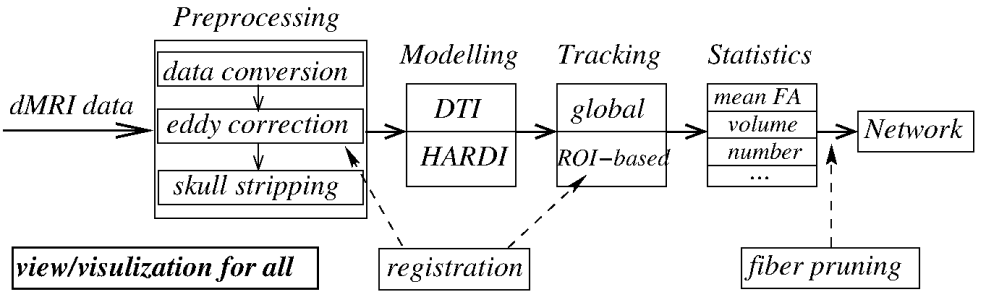
\includegraphics{overall.png}
\caption{Figure 1. The overall design framework of Diffusion Kit}\end{figure}
\begin{figure}[htbp]
\centering
\capstart

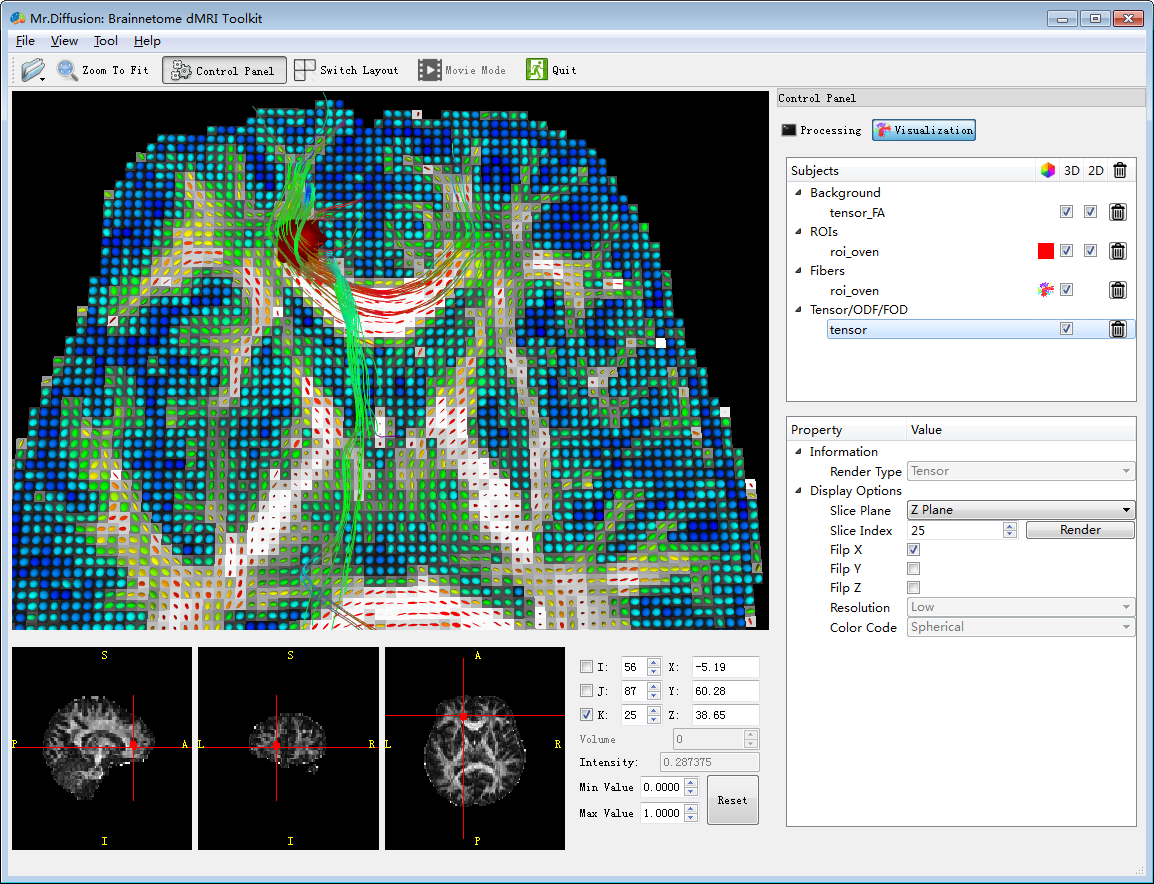
\includegraphics{mainwindow.png}
\caption{Figure 2. The main window of the software.}\end{figure}

It should be noteworthy that, for all the computing steps provided in GUI, the called commands with the complete parameter list are displayed in a separate log window. Such a design is special for the users to keep in mind what he/she is doing, and furthermore, it could be directly copied into script (Bash, Python …) for batch processing.
Preprocessing
\begin{figure}[htbp]
\centering
\capstart

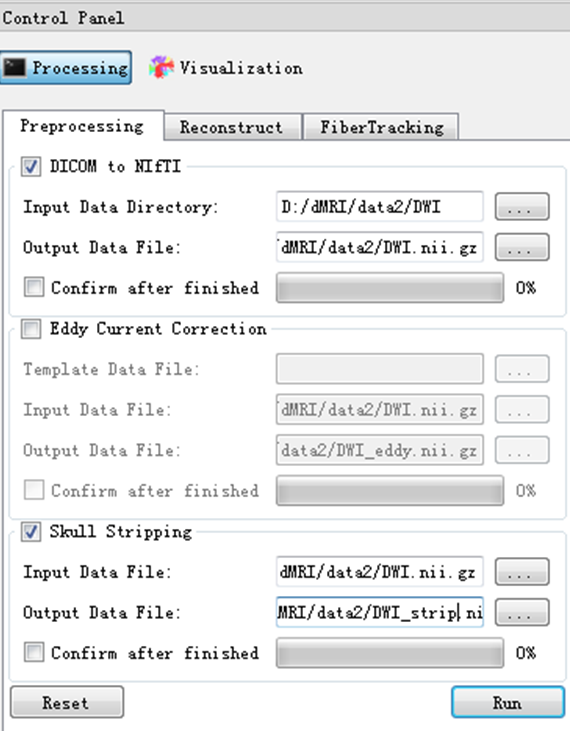
\includegraphics{preprocessing.png}
\caption{Figure 3. Data preprocessing steps, including data format conversion, eddy current correction and brain extraction.}\end{figure}

DICOM to NIFTI as unified data format

For saving space of data store, the nii.gz format was used throughout the whole pipeline. Firstly, we use the dcm2nii (by Chris Rorden, \href{https://www.nitrc.org/projects/dcm2nii}{https://www.nitrc.org/projects/dcm2nii}) to convert the data into a single 3/4D .nii.gz volume-series file, plus bval and bvec files. The format of bval file is

\begin{Verbatim}[commandchars=\\\{\}]
0 1500 1500 …… 1500
\end{Verbatim}

and the format of bvec file is

\begin{Verbatim}[commandchars=\\\{\}]
0  0.99944484233856   0.00215385644697   0.00269041745923 ...
0  \PYGZhy{}0.0053533311002   0.99836695194244   0.60518479347229 ...
0  0.03288444131613  \PYGZhy{}0.05708565562963   \PYGZhy{}0.79608047008514 ...
\end{Verbatim}

where the 0 in the first column indicates the b0 images in the scan and certainly the software also supports multi-b0 images. Since the DICOM formats from different scanner might be different, this function is not always able to successfully extract the bvec/bval files. If you encounter such a problem, please get back to us \textless{}link\textgreater{} and give the link of your data if it has big size beyond the email capability.

\begin{Verbatim}[commandchars=\\\{\}]
ccm@:bin\PYGZdl{} ./dcm2nii \PYGZhy{}h
Compression will be faster with /usr/local/bin/pigz
Chris Rorden\PYGZsq{}s dcm2niiX version 24Nov2014
usage: dcm2nii [options] \PYGZlt{}in\PYGZus{}folder\PYGZgt{}
 Options :
  \PYGZhy{}h : show help
  \PYGZhy{}f : filename (\PYGZpc{}c=comments \PYGZpc{}f=folder name \PYGZpc{}p=protocol \PYGZpc{}i ID of patient \PYGZpc{}n=name of patient \PYGZpc{}s=series, \PYGZpc{}t=time; default \PYGZsq{}DTI\PYGZsq{})
  \PYGZhy{}o : output directory (omit to save to input folder)
  \PYGZhy{}z : gz compress images (y/n, default n)
Defaults file : /home/ccm/.dcm2nii.ini
Examples :
 dcm2nii /Users/chris/dir
 dcm2nii \PYGZhy{}o /users/cr/outdir/ \PYGZhy{}z y \PYGZti{}/dicomdir
 dcm2nii \PYGZhy{}f mystudy\PYGZpc{}s \PYGZti{}/dicomdir
 dcm2nii \PYGZhy{}o \PYGZdq{}\PYGZti{}/dir with spaces/dir\PYGZdq{} \PYGZti{}/dicomdir
Example output filename: \PYGZsq{}/DTI.nii.gz\PYGZsq{}
\end{Verbatim}


\subsection{Data Processing Pipeline}
\label{userguide::doc}\label{userguide:data-processing-pipeline}

\subsubsection{Eddy and motion correction}
\label{userguide:eddy-and-motion-correction}
During the MRI scanning, many factors can cause magnetic field inhomogeneity, including changing magnetic fields from the imaging gradients and the radiofrequency (RF) coils and yielded biological effects. These effects usually degrade the imaging quality, resulting in artifacts including shearing and blurring (\href{http://mri-q.com/eddy-current-problems.html}{http://mri-q.com/eddy-current-problems.html}). Another type of artifacts is caused by head motion. Most of the artifacts described above could be amended by post-processing. In the eddy correction module, we apply a rigid registration method to address most of the shearing and motion artifacts. For the blurring artifacts, it still needs further investigation. Additional solutions would be added to reduce the magnetic field inhomogeneity by field mapping.

\begin{Verbatim}[commandchars=\\\{\}]
ccm@:bin\PYG{n+nv}{\PYGZdl{} }./bneddy \PYGZhy{}h
bneddy: Head Motion Correction.
   \PYGZhy{}i                                        Input file.
   \PYGZhy{}o                                        Output file.
   \PYGZhy{}ref             \PYG{l+m}{0}                       Indicating which frame is the reference.
\end{Verbatim}


\subsubsection{Brain stripping}
\label{userguide:brain-stripping}
This module is to strip the brain skull and extract the brain tissue, including gray matter, white matter, cerebrospinal fluid (CSF) and cerebellum. It largely benefits the following processing and analysis, offering better registration/alignment results and reducing computational time by excluding non-brain tissue. Therefore, although this step is not compulsory, we strongly recommend enforcing it. This module is adapted from the FSL/BET functions (\href{http://fsl.fmrib.ox.ac.uk/fsl/fslwiki/BET}{http://fsl.fmrib.ox.ac.uk/fsl/fslwiki/BET}) for its excellent efficacy and efficiency.

\begin{Verbatim}[commandchars=\\\{\}]
ccm@:bin\PYGZdl{} ./bet2 \PYGZhy{}h
Part of FSL (build 504)
BET (Brain Extraction Tool) v2.1 \PYGZhy{} FMRIB Analysis Group, Oxford
Usage:
bet2 \PYGZlt{}input\PYGZus{}fileroot\PYGZgt{} \PYGZlt{}output\PYGZus{}fileroot\PYGZgt{} [options]
Optional arguments (You may optionally specify one or more of):
       \PYGZhy{}o,\PYGZhy{}\PYGZhy{}outline    generate brain surface outline overlaid onto original image
       \PYGZhy{}m,\PYGZhy{}\PYGZhy{}mask \PYGZlt{}m\PYGZgt{}   generate binary brain mask
       \PYGZhy{}s,\PYGZhy{}\PYGZhy{}skull      generate approximate skull image
       \PYGZhy{}n,\PYGZhy{}\PYGZhy{}nooutput   don\PYGZsq{}t generate segmented brain image output
       \PYGZhy{}f \PYGZlt{}f\PYGZgt{}          fractional intensity threshold (0\PYGZhy{}\PYGZgt{}1); default=0.5; smaller values give larger brain outline estimates
       \PYGZhy{}g \PYGZlt{}g\PYGZgt{}          vertical gradient in fractional intensity threshold (\PYGZhy{}1\PYGZhy{}\PYGZgt{}1); default=0; positive values give larger brain outline at bottom, smaller at top
       \PYGZhy{}r,\PYGZhy{}\PYGZhy{}radius \PYGZlt{}r\PYGZgt{} head radius (mm not voxels); initial surface sphere is set to half of this
       \PYGZhy{}w,\PYGZhy{}\PYGZhy{}smooth \PYGZlt{}r\PYGZgt{} smoothness factor; default=1; values smaller than 1 produce more detailed brain surface, values larger than one produce smoother, less detailed surface
       \PYGZhy{}c \PYGZlt{}x y z\PYGZgt{}      centre\PYGZhy{}of\PYGZhy{}gravity (voxels not mm) of initial mesh surface.
       \PYGZhy{}t,\PYGZhy{}\PYGZhy{}threshold  \PYGZhy{}apply thresholding to segmented brain image and mask
       \PYGZhy{}e,\PYGZhy{}\PYGZhy{}mesh       generates brain surface as mesh in vtk format
       \PYGZhy{}v,\PYGZhy{}\PYGZhy{}verbose    switch on diagnostic messages
       \PYGZhy{}h,\PYGZhy{}\PYGZhy{}help       displays this help, then exits
\end{Verbatim}


\subsubsection{Reconstruction of the diffusion model}
\label{userguide:reconstruction-of-the-diffusion-model}
The reconstruction for diffusion model within pixels is one of the key topics in diffusion MRI research and it is also one of key modules of the software. At the current stage, we have integrated three modeling methods: one is the traditional Gaussian model (commonly known as DTI, diffusion tensor imaging), and the other two are for high angular resolution diffusion imaging (HARDI). For more detailed information please refer to our review paper {[}11,13{]}\_.


\paragraph{DTI reconstruction}
\label{userguide:dti-reconstruction}
The classical diffusion gradient sequence used in dMRI is the pulsed gradient spin-echo (PGSE) sequence proposed by Stejskal and Tanner. This sequence has 90o and 180o gradient pulses with duration time \(\delta\) and separation time \(\Delta\). To eliminate the dependence of spin density, we need at least two measurements of diffusion weighted imaging (DWI) signals, i.e. S(b) with the diffusion weighting factor b in Eq. (1) introduced by Le Bihan etc, and S(0) with b = 0 which is the baseline signal without any gradient.

In the b-value in Eq. (1), \$\textbackslash{}gamma\$ is the proton gyromagnetic ratio, \$\textbackslash{}bf\{G\}=\textbar{}\textbar{}\textbackslash{}bf\{G\}\textbar{}\textbar{}\textbackslash{}bf\{u\}\$ is the diffusion sensitizing gradient pulse with norm \$\textbar{}\textbar{}\{\textbackslash{}bf G\}\textbar{}\textbar{}\$ and direction \$\{\textbackslash{}bf u\}\$. \$\textbackslash{}tau=\textbackslash{}Delta-\textbackslash{}frac\{1\}\{3\}\textbackslash{}delta\$ is normally used to describe the effective diffusion time. Using the PGSE sequence with S(b), the diffusion weighted signal attenuation E(b) is given by Stejskal-Tanner equation,

where D is known as the apparent diffusion coefficient (ADC) which reflects the property of surrounding tissues. Note that in general ADC D is also dependent on G in a complex way. However, free diffusion in DTI assumes D is only dependent on the direction of G, i.e. . The early works in dMRI reported that ADC D is dependent on gradient direction u and used two or three DWI images in different directions to detect the properties of tissues. Then Basser et al. introduced diffusion tensor \footnote{
Basser P.J., Mattiello J., LeBihan D., MR diffusion tensor spectroscopy and imaging. Biophysical journal, 1994. 66, 259-267.
} to represent ADC as \$D(\textbackslash{}bf\{u\}) = \{\textbackslash{}bf u\textasciicircum{}\{T\}\}\{\textbackslash{}bf D\}\textbackslash{}bf\{u\}\$, where \$\{\textbackslash{}bf D\}\$ is called as the diffusion tensor, which is a 3 × 3 symmetric positive definite matrix independent of u. This method is called as diffusion tensor imaging (DTI) and is the most common method nowadays in dMRI technique. In DTI, the signal E(b) is represented as
\begin{figure}[htbp]
\centering
\capstart

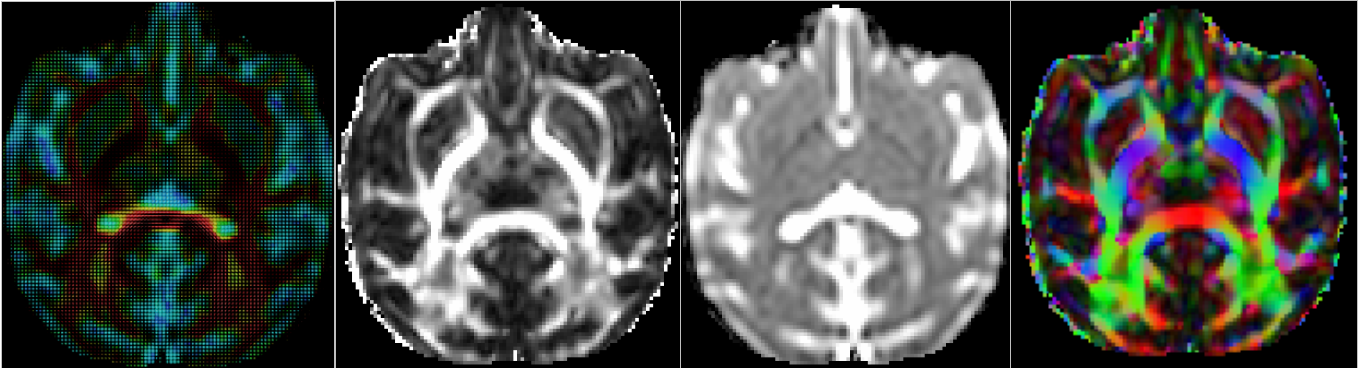
\includegraphics{scalarmaps.png}
\caption{Figure 4. Tensor field and the scalar maps estimated from a monkey data with b = 1500s/mm2.}\end{figure}

The diffusion tensor D can be estimated from measured diffusion signal samples  through a simple least square method or weighted least square method \footnotemark[12], or more complex methods that consider positive definite constraint or Rician noise. If single b-value is used, the optimal b-value for tensor estimation was reported to in the range of (0.7, 1.5) × 10−3 s/mm2, and normally about twenty DWI images are used in DTI in clinical study. ome useful indices can be obtained from tensor D. The most important three indices are fractional anisotropy (FA), mean diffusivity (MD) and relative anisotropy (RA) defined as

where,  are the three eigenvalues of D and  is the mean eigenvalue. MD and FA have been used in many clinical applications. For example, MD is known to be useful in stroke study. For more detailed information please refer to our review paper \footnote{
Zuo N., Cheng J., Jiang T., 2012. Diffusion magnetic resonance imaging for Brainnetome: A critical review, Neuroscience bulletin, DOI: 10.1007/s12264-012-1245-3.
}.

\begin{Verbatim}[commandchars=\\\{\}]
ccm@:bin\PYG{n+nv}{\PYGZdl{} }./bndti\PYGZus{}estimate \PYGZhy{}h
bndti\PYGZus{}estimate: Diffusion Tensors Estimation.
MR. Diffusion \PYG{o}{(}v1.0\PYG{o}{)}, http://www.brainnetome.org/en/brat.html.
\PYG{o}{(}Oct  \PYG{l+m}{9} 2015, 19:26:40\PYG{o}{)}
general arguments
   \PYGZhy{}d                                Input DWI Data, in NIFTI/Analyze format \PYG{o}{(}4D\PYG{o}{)}
   \PYGZhy{}g                                Gradients direction file
   \PYGZhy{}b                                b value file
   \PYGZhy{}m                                Brain mask : filein mask \PYG{p}{\textbar{}} OPTIONAL
   \PYGZhy{}o                                Result DTI : fileout DTI
   \PYGZhy{}tensor          \PYG{l+m}{0}                Save tensor : \PYG{l+m}{0} \PYGZhy{} No\PYG{p}{;} \PYG{l+m}{1} \PYGZhy{} Yes\PYG{p}{;} \PYG{o}{(}Default: 0\PYG{o}{)}
   \PYGZhy{}eig             \PYG{l+m}{0}                Save eigenvalues and eigenvectors : \PYG{l+m}{0} \PYGZhy{} No\PYG{p}{;} \PYG{l+m}{1} \PYGZhy{} Yes\PYG{p}{;} \PYG{o}{(}Default: 0\PYG{o}{)}
\end{Verbatim}


\paragraph{SPFI reconstruction}
\label{userguide:spfi-reconstruction}
It was proposed that the SPFI method has more powerful capability to identify the tangling fibers \footnote{
Cheng J, Jiang T, Deriche R. Nonnegative definite EAP and ODF estimation via a unified multi-shell HARDI reconstruction. Med Image Comput Comput Assist Interv., 15(Pt 2):313-21, 2012.
}. In SPFI \footnotemark[8], the diffusion signal  is represented by spherical polar Fourier (SPF) basis functions in Eq. 7.

The SPF basis denoted by  is a 3D orthonormal basis with spherical harmonics in the spherical portion and the Gaussian-Laguerre function in the radial portion. Furthermore, Cheng and his colleagues proposed a uniform analytical solution to transform the coefficients  of  to the coefficients  of ODF (orientation distribution function) represented by the spherical harmonics basis, as in Eq. 8.

It is a model-free, regularized, fast and robust reconstruction method which can be performed with single-shell or multiple-shell HARDI data to estimate the ODF proposed by Wedeen et al. \footnote{
Wedeen V.J., Hagmann P., Tseng W.Y., Reese T.G., Weisskoff R.M., 2005. Mapping complex tissue architecture with diffusion spectrum magnetic resonance imaging. Magn Reson Med, 54(6):1377-1386.
}. The implementation of analytical SPFI includes two independent steps. The first estimates the coefficients of  with least squares, and the second transforms the coefficients of  to the coefficients of ODF.

\begin{Verbatim}[commandchars=\\\{\}]
ccm@:bin\PYG{n+nv}{\PYGZdl{} }bnhardi\PYGZus{}ODF\PYGZus{}estimate \PYGZhy{}h
bnhardi\PYGZus{}ODF\PYGZus{}estimate: Orientation Distribution Function Estimation \PYG{o}{(}SPFI method\PYG{o}{)}.
MR. Diffusion \PYG{o}{(}v1.0\PYG{o}{)}, http://www.brainnetome.org/en/brat.html.
\PYG{o}{(}Jul \PYG{l+m}{15} 2015, 11:50:20\PYG{o}{)}
  \PYGZhy{}d                                        dwi data
  \PYGZhy{}b                                        text file contains b\PYGZhy{}value
  \PYGZhy{}g                                        text file contains grad direction
  \PYGZhy{}m                                        Brain mask.
  \PYGZhy{}o                                        output odf file
  \PYGZhy{}scale           \PYGZhy{}1                       \PYG{k}{if} not given, a suggested scheme is used
  \PYGZhy{}tau             0.02533                  tar value to calculate the \PYG{n+nb}{true }pdf.
  \PYGZhy{}b0\PYGZus{}w            \PYG{l+m}{1}                        b0 weight \PYG{k}{for} the least square estimate
  \PYGZhy{}b0\PYGZus{}analytical   \PYG{l+m}{1}                        \PYG{n+nb}{true}: analytical
  \PYGZhy{}is\PYGZus{}assemlal     \PYG{n+nb}{true                     }\PYG{n+nb}{true}: assemlal basis\PYG{p}{;} \PYG{n+nb}{false}: cheng basis
  \PYGZhy{}outGFA          \PYG{n+nb}{false                    }output GFA: \PYG{n+nb}{true }or \PYG{n+nb}{false}
  \PYGZhy{}rdis            0.015                    r value \PYG{k}{for} pdf.
  \PYGZhy{}sh              \PYG{l+m}{4}                        order of spherical harmonics
  \PYGZhy{}ra              \PYG{l+m}{1}                        order of radial part
  \PYGZhy{}lambda\PYGZus{}sh       \PYG{l+m}{0}                        regualrization parameter \PYG{k}{for} sh basis
  \PYGZhy{}lambda\PYGZus{}ra       \PYG{l+m}{0}                        regualrization parameter \PYG{k}{for} ra basis
\end{Verbatim}


\paragraph{CSD reconstruction}
\label{userguide:csd-reconstruction}
The CSD method was proposed by Tournier et al. \footnote{
Tournier JD, Calamante F, Connelly A. Robust determination of the fibre orientation distribution in diffusion MRI: non-negativity constrained super-resolved spherical deconvolution. Neuroimage, 35 (4): 1459-1472, 2007.
}, which expresses the diffusion signal as in Eq. 9,

where  is called the fiber orientation density function (fODF), which needs to be estimated, and  is the response function, which is the typical signal generated from one fiber. The response function can be directly estimated from diffusion weighted image (DWI) data by measuring the diffusion profile in the voxels with the highest fractional anisotropy values, indicating that a single coherently oriented fiber population is contained in these voxels. When the response function is obtained, we can utilize the deconvolution of  from  to estimate the fiber ODF. The computation of the fiber ODF was carried out using the software MRtrix (J-D Tournier, Brain Research Institute, Melbourne, Australia, \href{http://www.brain.org.au/software/}{http://www.brain.org.au/software/}). We thank Dr. Jacques-Donald Tournier for sharing MATLAB code of the CSD method, which inspired a quick C/C++ implementation.

\begin{Verbatim}[commandchars=\\\{\}]
ccm@:bin\PYG{n+nv}{\PYGZdl{} }./bnhardi\PYGZus{}FOD\PYGZus{}estimate \PYGZhy{}h
bnhardi\PYGZus{}FOD\PYGZus{}estimate: Constraind Spherical Deconvolution \PYG{o}{(}CSD\PYG{o}{)} based HARDI reconstruciton.
MR. Diffusion \PYG{o}{(}v1.0\PYG{o}{)}, http://www.brainnetome.org/en/brat.html.
\PYG{o}{(}Jul \PYG{l+m}{15} 2015, 11:50:20\PYG{o}{)}
general arguments
   \PYGZhy{}d                                        Input DWI Data, in NIFTI/Analyze format \PYG{o}{(}4D\PYG{o}{)}
   \PYGZhy{}g                                        Gradients direction file
   \PYGZhy{}b                                        b value file
   \PYGZhy{}m                                        Brain mask : filein mask \PYG{p}{\textbar{}} OPTIONAL
   \PYGZhy{}outFA           \PYG{l+m}{1}                        Whether to output the FA of DTI
   \PYGZhy{}o                                        Result CSD Estimate \PYG{o}{(}.nii.gz\PYG{o}{)}
   \PYGZhy{}lmax            \PYG{l+m}{8}                        6/8/10, Max order of the adopted harmonical base
   \PYGZhy{}fa              \PYG{o}{[}0.75,0.95\PYG{o}{]}              The FA thesshold considered as single fiber
   \PYGZhy{}erode           \PYGZhy{}1                       The unit is voxel: Remove the garbage near the boundary of FA image, \PYG{k}{for} better estimating response \PYG{k}{function}
   \PYGZhy{}nIter           \PYG{l+m}{50}                       Max iteration number before aborting
   \PYGZhy{}lambda          \PYG{l+m}{1}                        The regularization weight \PYG{k}{for} optimization
   \PYGZhy{}tau             0.1                      The threshold on the FOD amplitude used to identify negative lobes
   \PYGZhy{}hr             \PYG{l+m}{300}                      300/1000/5000. The later get more acurate estimation \PYG{k}{while} more \PYG{n+nb}{time }consuming, so use the first one unless your computer is powerful !
\end{Verbatim}


\subsubsection{Fiber tracking and attributes extraction}
\label{userguide:fiber-tracking-and-attributes-extraction}
Fiber tracking is a critical way to construct the anatomical connectivity matrix. For the tracking based on tensors from DTI, an intuitive way is to link the neighboring voxels following their main directions (e.g. V1 in the eigenvector of the DTI) given a set of some stop criteria, such as maximum bending angle of the curve and minimum FA value, which is to ensure the target voxel is indeed white matter microstructure. This is the so called deterministic streamline tractography \footnote{
Alexander, A.L., Lee, J.E., Lazar, M., Field, A.S., 2007. Diffusion tensor imaging of the brain. Neurotherapeutics 4, 316-329.
}, as illustrated in Figure 5.
\begin{figure}[htbp]
\centering
\capstart

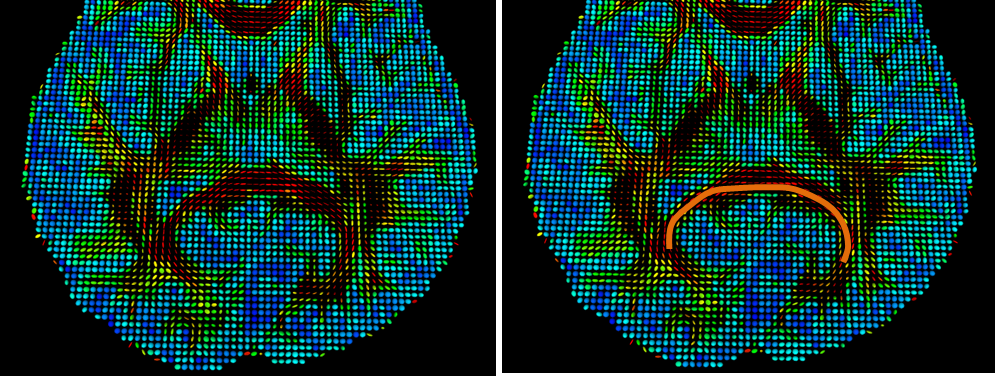
\includegraphics{tractography.png}
\caption{Figure 5. Illustration for deterministic streamline tractography.}\end{figure}

\begin{Verbatim}[commandchars=\\\{\}]
ccm@:bin\PYG{n+nv}{\PYGZdl{} }./bndti\PYGZus{}tracking \PYGZhy{}h
bndti\PYGZus{}tracking: DTI Deterministic Fibertracking.
MR. Diffusion \PYG{o}{(}v1.0\PYG{o}{)}, http://www.brainnetome.org/en/brat.html.
\PYG{o}{(}Oct  \PYG{l+m}{9} 2015, 19:26:46\PYG{o}{)}
   \PYGZhy{}d                                        Input DTI data.
   \PYGZhy{}m                                        Mask Image.
   \PYGZhy{}s                                        Seeds Image.
   \PYGZhy{}fa                                       FA Image.
   \PYGZhy{}ft              0.1                      FA Threshold
   \PYGZhy{}at              \PYG{l+m}{45}                       Angular Threshold.
   \PYGZhy{}sl              0.5                      Step Length \PYG{o}{(}Voxel\PYG{o}{)}.
   \PYGZhy{}min             \PYG{l+m}{10}                       Threshold the fiber \PYG{o}{(}mm\PYG{o}{)}. \PYG{o}{(}remove fibers shorter than the number\PYG{o}{)}
   \PYGZhy{}max             \PYG{l+m}{5000}                     Upper\PYGZhy{}threshold the fiber \PYG{o}{(}mm\PYG{o}{)}. \PYG{o}{(}remove fibers longer than the number\PYG{o}{)}
   \PYGZhy{}o                                        Output Fibers Filename \PYG{o}{(}.fiber file\PYG{o}{)}.
\end{Verbatim}

The tracking module in the software for HARDI estimation is similar to the streamline method as described above. It should be kept in mind that, for HARDI estimation, usually there are more than one main direction (which is what we desired since it possibly identifies tangling fibers), so we should consider these kissing/branching cases. Meanwhile, since there is no explicit dominant directions for each voxel, searching algorithm should be applied to locate the main directions. The searching should run for each voxel, so it is not as fast as the traditional DTI tracking.

\begin{Verbatim}[commandchars=\\\{\}]
ccm@:bin\PYG{n+nv}{\PYGZdl{} }./bnhardi\PYGZus{}tracking \PYGZhy{}h
bnhardi\PYGZus{}tracking: HARDI Deterministic Fibertracking.
Mr. Diffusion \PYG{o}{(}v1.0\PYG{o}{)}, http://www.brainnetome.org/en/brat.html.
\PYG{o}{(}Oct  \PYG{l+m}{9} 2015, 19:26:46\PYG{o}{)}
   \PYGZhy{}d                                        HARDI spherical harmonic image.
   \PYGZhy{}a                                        Anisotropy image.
   \PYGZhy{}m                                        Mask file.
   \PYGZhy{}s                                        Seeds file.
   \PYGZhy{}o                                        Fiber file \PYG{o}{(}.fiber file\PYG{o}{)}.
   \PYGZhy{}sl              0.5                      Step length \PYG{o}{(}Voxel\PYG{o}{)}: float
   \PYGZhy{}ft              0.1                      FA threshold: float
   \PYGZhy{}at              \PYG{l+m}{75}                       Angle threshold: float
   \PYGZhy{}min             \PYG{l+m}{10}                       Threshold the fiber \PYG{o}{(}mm\PYG{o}{)}. \PYG{o}{(}remove fibers shorter than the number\PYG{o}{)}
   \PYGZhy{}max             \PYG{l+m}{5000}                    Upper\PYGZhy{}threshold the fiber \PYG{o}{(}mm\PYG{o}{)}. \PYG{o}{(}remove fibers longer than the number\PYG{o}{)}
\end{Verbatim}


\subsubsection{Visualization for various images}
\label{userguide:visualization-for-various-images}
The software provides a variety of entries for visualizing different data types, including 3D/4D image, Tensor/ODF/FOD image and white mater fibers. The views of different data could be superimposed for a precise anatomical localization. It should be noted that, if one uses the GUI, these view functions could be called in each processing steps for inspecting the results.

Figure 6. Illustrations for the capability of the software to show many types of images.

\begin{Verbatim}[commandchars=\\\{\}]
ccm@:bin\PYG{n+nv}{\PYGZdl{} }./bnviewer \PYGZhy{}h
This program is the GUI frontend that displays and performs data reconstruction and fiber tracking on diffusion MR images, which have been developed by the teams of Brainnetome Center, CASIA.
basic usage:
  bnviewer \PYG{o}{[}\PYG{o}{[}\PYGZhy{}volume\PYG{o}{]} DTI\PYGZus{}FA.nii.gz\PYG{o}{]}
           \PYG{o}{[}\PYGZhy{}roi ROI/roi\PYGZus{}cc\PYGZus{}top.nii.gz\PYG{o}{]}
           \PYG{o}{[}\PYGZhy{}fiber ROI/roi\PYGZus{}cc\PYGZus{}top.fiber\PYG{o}{]}
           \PYG{o}{[}\PYGZhy{}tensor DTI.nii.gz\PYG{o}{]}/\PYG{o}{[}\PYGZhy{}odf HARDI.nii.gz\PYG{o}{]}
           \PYG{o}{[}\PYGZhy{}atlas DTI.nii.gz\PYG{o}{]}
options:
  \PYGZhy{}help                  show this \PYG{n+nb}{help}
  \PYGZhy{}volume  .nii.gz       \PYG{n+nb}{set }input background data
  \PYGZhy{}roi     .nii.gz       \PYG{n+nb}{set }input ROI data
  \PYGZhy{}fiber   .fiber/.trk   \PYG{n+nb}{set }input fiber data
  \PYGZhy{}tensor  .nii.gz       \PYG{n+nb}{set }input DTI data \PYG{o}{(}conflict with \PYGZhy{}odf args\PYG{o}{)}
  \PYGZhy{}odf     .nii.gz       \PYG{n+nb}{set }input ODF/FOD data \PYG{o}{(}conflict with \PYGZhy{}tensor args\PYG{o}{)}
\end{Verbatim}


\subsubsection{Several other useful tools}
\label{userguide:several-other-useful-tools}

\paragraph{Image registration}
\label{userguide:image-registration}
This module is implemented by elastix \footnote{
\href{http://elastix.isi.uu.nl/}{http://elastix.isi.uu.nl/}
}, which integrates a collection of functions from ITK \footnote{
\href{http://www.itk.org}{http://www.itk.org}
}. In our software, the registration module is customized to auto-configure the parameter settings between different image modalities, e.g., two DWI images (for eddy current correction in current version), standard space and T1 space (for mapping ROIs to the individual space), DWI space and standard space (for statistical comparisons across subjects). This module contains two separate submodules, \textless{}code\textgreater{}elastix\textless{}/code\textgreater{} for computing the transform matrix and \textless{}code\textgreater{}transformix\textless{}/code\textgreater{} for applying the existing transform matrix to an image.

\begin{Verbatim}[commandchars=\\\{\}]
ccm@:bin\PYG{n+nv}{\PYGZdl{} }./elastix \PYGZhy{}h
elastix version: 4.700
elastix registers a moving image to a fixed image.
The registration\PYGZhy{}process is specified in the parameter file.
 \PYGZhy{}\PYGZhy{}help, \PYGZhy{}h displays this message and \PYG{n+nb}{exit}
 \PYGZhy{}\PYGZhy{}version  output version information and \PYG{n+nb}{exit}
Call elastix from the \PYG{n+nb}{command }line with mandatory arguments:
 \PYGZhy{}f        fixed image
 \PYGZhy{}m        moving image
 \PYGZhy{}out      output directory
 \PYGZhy{}p        parameter file, elastix handles \PYG{l+m}{1} or more \PYG{l+s+s2}{\PYGZdq{}\PYGZhy{}p\PYGZdq{}}
Optional extra commands:
 \PYGZhy{}fMask    mask \PYG{k}{for} fixed image
 \PYGZhy{}mMask    mask \PYG{k}{for} moving image
 \PYGZhy{}t0       parameter file \PYG{k}{for} initial transform
 \PYGZhy{}priority \PYG{n+nb}{set }the process priority to high, abovenormal, normal \PYG{o}{(}default\PYG{o}{)},
           belownormal, or idle \PYG{o}{(}Windows only option\PYG{o}{)}
 \PYGZhy{}threads  \PYG{n+nb}{set }the maximum number of threads of elastix
\end{Verbatim}

The parameter-file must contain all the information necessary for elastix to runproperly. That includes which metric to use, which optimizer, which transform, etc. It must also contain information specific for the metric, optimizer, transform, etc. For a usable parameter-file, see the website.


\subparagraph{Need further help?}
\label{userguide:need-further-help}
Check the website \href{http://elastix.isi.uu.nl}{http://elastix.isi.uu.nl}, or mail \href{mailto:elastix@bigr.nl}{elastix@bigr.nl}.

\begin{Verbatim}[commandchars=\\\{\}]
ccm@:bin\PYG{n+nv}{\PYGZdl{} }./transformix \PYGZhy{}h
transformix version: 4.700
transformix applies a transform on an input image and/or generates a deformation field.
The transform is specified in the transform\PYGZhy{}parameter file.
 \PYGZhy{}\PYGZhy{}help, \PYGZhy{}h displays this message and \PYG{n+nb}{exit}
 \PYGZhy{}\PYGZhy{}version  output version information and \PYG{n+nb}{exit}
\end{Verbatim}

Call transformix from the command line with mandatory arguments:
\begin{optionlist}{3cm}
\item [-out]  
output directory
\item [-tp]  
transform-parameter file, only 1
\end{optionlist}

Optional extra commands:
\begin{optionlist}{3cm}
\item [-in]  
input image to deform
\item [-def]  
file containing input-image points; the point are transformed
according to the specified transform-parameter file
use ``-def all'' to transform all points from the input-image, which
effectively generates a deformation field.
\item [-jac]  
use ``-jac all'' to generate an image with the determinant of the
spatial Jacobian
\item [-jacmat]  
use ``-jacmat all'' to generate an image with the spatial Jacobian
matrix at each voxel
\item [-priority]  
set the process priority to high, abovenormal, normal (default),
belownormal, or idle (Windows only option)
\item [-threads]  
set the maximum number of threads of transformix
\end{optionlist}

At least one of the options ``-in'', ``-def'', ``-jac'', or ``-jacmat'' should be given.

The transform-parameter file must contain all the information necessary for transformix to run properly. That includes which transform to use, with which parameters, etc. For a usable transform-parameter file, run elastix, and inspect the output file ``TransformParameters.0.txt''.


\paragraph{Image calculation and ROI generation}
\label{userguide:image-calculation-and-roi-generation}
The module bncalc provides simple image calculations, such as add/minus/multiply/divide operations. Meanwhile, it can also generate user-defined ROIs given the origin and radius in a user-specified image space.

\begin{Verbatim}[commandchars=\\\{\}]
ccm@:bin\PYG{n+nv}{\PYGZdl{} }./bncalc \PYGZhy{}h
Mr. Diffusion \PYG{o}{(}v1.0\PYG{o}{)}, http://www.brainnetome.org/en/brat.html.
This funciton provide basic process \PYG{k}{for} the input data \PYG{o}{(}NIFTI/Analyze format\PYG{o}{)}
Usage of bncalc:
   \PYGZhy{}i       image         The original file you want to manage.
   \PYGZhy{}add     image/value   Add to the data from the last step.
   \PYGZhy{}sub     image/value   Subtract data from the last step.
   \PYGZhy{}mul     image/value   Multiply the data from the last step.
   \PYGZhy{}div     image/value   Divide the data from the last step.
   \PYGZhy{}roi     x,y,z,r       Generate a ROI centered at \PYG{o}{[}x,y,z\PYG{o}{]}\PYG{o}{(}MNI mm\PYG{o}{)} with radius r,
                          in the input data space.
   \PYGZhy{}mask    image         Mask the data from last step by this input one.
                          If this input is a binary, \PYG{k}{then} it is the same as
                          \PYGZhy{}mul, otherwise it keep the voxels from the last step
                          when the new input is nonzero.
   \PYGZhy{}bin     value         \PYG{n+nb}{set }\PYG{l+m}{1} \PYG{k}{if} \PYGZgt{}value, otherwise 0.
   \PYGZhy{}uthr    value         Set \PYG{n+nv}{voxel}\PYG{o}{=}\PYG{l+m}{0} when it\PYGZgt{}\PYG{o}{=}value.
   \PYGZhy{}dthr    value         Set \PYG{n+nv}{voxel}\PYG{o}{=}\PYG{l+m}{0} when it\PYGZlt{}\PYG{o}{=}value.
   \PYGZhy{}o       image         output a NIFTI \PYG{o}{(}.nii.gz\PYG{o}{)} file
\end{Verbatim}


\paragraph{Fiber manipulation}
\label{userguide:fiber-manipulation}
After obtaining a large bundle of white matter fibers, you may want to prune the fibers that go through specified locations (ROIs). Here, we provide several tools to manipulate the fiber bundles.
bnfiber\_manipulate, to split/merge fiber bundles based on given ROIs.

\begin{Verbatim}[commandchars=\\\{\}]
bnfiber\PYGZus{}manipulate: Merge or prune fiber bundles based on given ROIs.
Mr. Diffusion \PYG{o}{(}v1.0\PYG{o}{)}, http://www.brainnetome.org/en/brat.html.
\PYG{o}{(}Sep \PYG{l+m}{17} 2015, 14:47:12\PYG{o}{)}
   \PYGZhy{}fiber                                    fiber file
   \PYGZhy{}and                                      AND file: ro1.nii.gz,roi2.nii.gz
   \PYGZhy{}or                                       OR file: roi1.nii.gz,roi2.nii.gz
   \PYGZhy{}not                                      NOT file: ro1.nii.gz,roi2.nii.gz
   \PYGZhy{}o                                        Output file \PYG{o}{(}.fiber file\PYG{o}{)}.
\end{Verbatim}

bnfiber\_end, to cut the fiber bundles given start/stop ROIs, which is useful to get the exact connections between two ROIs in constructing connectivity matrix.

\begin{Verbatim}[commandchars=\\\{\}]
ccm@:bin\PYG{n+nv}{\PYGZdl{} }./bnfiber\PYGZus{}end \PYGZhy{}h
bnfiber\PYGZus{}end: Extract fibers which end in the two given rois.Mr. Diffusion \PYG{o}{(}v1.0\PYG{o}{)}, http://www.brainnetome.org/en/brat.html.
\PYG{o}{(}Sep \PYG{l+m}{17} 2015, 14:47:12\PYG{o}{)}
   \PYGZhy{}fiber                                    fiber file
   \PYGZhy{}roi1                                     roi1 file
   \PYGZhy{}roi2                                     roi2 file
   \PYGZhy{}o                                        Output file \PYG{o}{(}.fiber file\PYG{o}{)}
\end{Verbatim}

bnfiber\_stats, to extract statistical properties of the fiber bundle, such as mean FA/MD and fiber numbers.

\begin{Verbatim}[commandchars=\\\{\}]
ccm@:bin\PYG{n+nv}{\PYGZdl{} }./bnfiber\PYGZus{}stats \PYGZhy{}h
bnfiber\PYGZus{}stats: Show fiber stats.
Mr. Diffusion \PYG{o}{(}v1.0\PYG{o}{)}, http://www.brainnetome.org/en/brat.html.
\PYG{o}{(}Sep \PYG{l+m}{17} 2015, 14:47:12\PYG{o}{)}
   \PYGZhy{}fiber                                    Input fiber file, \PYG{k}{then} output mean FA/MD, number of fibers et al.
\end{Verbatim}

bnfiber\_map, to compute the fiber density map which is used in track density imaging \footnote{
Calamante F., Tournier J.D., Heidemann R.M., Anwander A., Jackson G.D., Connelly A., 2011. Track density imaging (TDI): validation of super resolution property. Neuroimage, 56, 1259-66.
}.

\begin{Verbatim}[commandchars=\\\{\}]
ccm@:bin\PYG{n+nv}{\PYGZdl{} }./bnfiber\PYGZus{}map \PYGZhy{}h
bnfiber\PYGZus{}map: Calculate the fiber density according to the reference volume.
Mr. Diffusion \PYG{o}{(}v1.0\PYG{o}{)}, http://www.brainnetome.org/en/brat.html.
\PYG{o}{(}Sep \PYG{l+m}{17} 2015, 14:47:13\PYG{o}{)}
   \PYGZhy{}fiber                                    Fiber file
   \PYGZhy{}ref                                      Reference file \PYG{o}{(}NIfTI\PYG{o}{)}
   \PYGZhy{}o                                        Output file \PYG{o}{(}NIfTI\PYG{o}{)}.
   \PYGZhy{}nor             \PYG{l+m}{1}                        Normalize fiber density: 1\PYG{o}{(}yes\PYG{o}{)} or 0\PYG{o}{(}no\PYG{o}{)}.
\end{Verbatim}

bnmerge/bnsplit, to merge the 3D volumes to 4D or split 4D to 3D volumes.

\begin{Verbatim}[commandchars=\\\{\}]
ccm@:bin\PYG{n+nv}{\PYGZdl{} }./bnmerge \PYGZhy{}h
bnmerge: Merge 3D NIfTI files  to 4D NIfTI file.
   This program is to merge 3D NIfTI files to 4D NIfTI file.
   Usage: bnmerge filein1 filein2 ... fileout
   options:     \PYGZhy{}h           : show this \PYG{n+nb}{help}
\end{Verbatim}

\begin{Verbatim}[commandchars=\\\{\}]
ccm@:bin\PYG{n+nv}{\PYGZdl{} }./bnsplit \PYGZhy{}h
bnsplit: Split 4D volume to 3D volumes.
   This program splits 4D volume to 3D volumes.
   basic usage: split \PYGZhy{}i FILE\PYGZus{}IN \PYGZhy{}o FILE\PYGZus{}OUT prefix
   options:     \PYGZhy{}h           : show this \PYG{n+nb}{help}
                \PYGZhy{}v LEVEL     : the verbose level to LEVEL
\end{Verbatim}

bninfo, to display a short head information of the input image. Supported input image format includes NIFTI/DICOM.

\begin{Verbatim}[commandchars=\\\{\}]
ccm@:DWI\PYG{n+nv}{\PYGZdl{} }bninfo \PYGZhy{}h
bninfo: Show file header information.
Mr. Diffusion \PYG{o}{(}v1.0\PYG{o}{)}, http://www.brainnetome.org/en/brat.html.
\PYG{o}{(}Jul \PYG{l+m}{15} 2015, 11:50:01\PYG{o}{)}
   \PYGZhy{}i                                        Nifti/ANALYZE/DICOM file.
\end{Verbatim}


\paragraph{Reference}
\label{userguide:reference}

\subsection{GUI Fornt-end of Data Processing Pipeline}
\label{frontend:gui-fornt-end-of-data-processing-pipeline}\label{frontend::doc}

\subsection{Guidelines on Data Visualization}
\label{visualization::doc}\label{visualization:guidelines-on-data-visualization}
In this page, the general functionality implemented in the \code{bnviewer} program is
described in detail. This covers methods that a user can visualize almost all kinds of
diffusion MRI data.

Except those specially noticed, all the data should be formatted in either NIFTI or
ANAYLYZE image. NIFTI format is recommended, see {\hyperref[fileformat:data-format]{\emph{\DUspan{}{Data Format}}}} page for more details.


\subsubsection{Command Line Interface}
\label{visualization:command-line-interface}
Typing \code{bnviewer -h} in command line would given following information, which
help users to load a list of files without click them one by one.
The can be extremely useful when one wants to contantly load a large list of data files
to get screen capture images.

\begin{Verbatim}[commandchars=\\\{\}]
basic uage:
  bnviewer \PYG{o}{[}\PYG{o}{[}\PYGZhy{}volume\PYG{o}{]} DTI\PYGZus{}FA.nii.gz\PYG{o}{]}
           \PYG{o}{[}\PYGZhy{}roi ROI/roi\PYGZus{}cc\PYGZus{}top.nii.gz\PYG{o}{]}
           \PYG{o}{[}\PYGZhy{}fiber ROI/roi\PYGZus{}cc\PYGZus{}top.fiber\PYG{o}{]}
           \PYG{o}{[}\PYGZhy{}tensor DTI.nii.gz\PYG{o}{]}/\PYG{o}{[}\PYGZhy{}odf HARDI.nii.gz\PYG{o}{]}
           \PYG{o}{[}\PYGZhy{}atlas DTI.nii.gz\PYG{o}{]}

options:
  \PYGZhy{}help                  show this \PYG{n+nb}{help}
  \PYGZhy{}volume  .nii.gz       \PYG{n+nb}{set }input background data
  \PYGZhy{}roi     .nii.gz       \PYG{n+nb}{set }input ROI data
  \PYGZhy{}fiber   .fiber/.trk   \PYG{n+nb}{set }input fiber data
  \PYGZhy{}tensor  .nii.gz       \PYG{n+nb}{set }input DTI data \PYG{o}{(}conflict with \PYGZhy{}odf args\PYG{o}{)}
  \PYGZhy{}odf     .nii.gz       \PYG{n+nb}{set }input ODF/FOD data \PYG{o}{(}conflict with \PYGZhy{}tensor args\PYG{o}{)}
\end{Verbatim}

\begin{notice}{note}{Todo}

create interface for generating high quality images and save them into specified location.
\end{notice}


\subsubsection{Image Data Navigation}
\label{visualization:image-data-navigation}

\paragraph{3D Navigation}
\label{visualization:d-navigation}
When an image data is loaded, one can change view angle by dragging \emph{left} mouse button.
This is the default interactor style implemented in \emph{vtkInteractorStyleTrackballCamera},
which is used internally in our program. According to VTK's documentation:
\begin{quote}

vtkInteractorStyleTrackballCamera allows the user to interactively manipulate
(rotate, pan, etc.) the camera, the viewpoint of the scene.
In trackball interaction, the magnitude of the mouse motion is proportional
to the camera motion associated with a particular mouse binding.
For example, small left-button motions cause small changes in the rotation of
the camera around its focal point. For a 3-button mouse, the left button
is for \emph{rotation}, the right button for \emph{zooming},
the middle button for \emph{panning} (translation),
and ctrl + left button for \emph{spinning}. (With fewer mouse buttons,
ctrl + shift + left button is for zooming, and shift + left button is for panning.)
\end{quote}

We simplify the trackball interaction to used middle button for both panning and zooming,
in order to spare right mouse click to popup option menu for more actions.

The \textbf{Background Color} for 3D view is defined as black by default.
This can be changed from option menu popped up when \emph{right} mouse click event is captured.
By selecting the color from the popup color dialog, the background color is changed instantly.


\paragraph{2D Navigation}
\label{visualization:id1}
Three 2D slice image views are placed below 3D view by default.
The three slice views from left to right are \emph{sagittal plane, coronal plane} and
\emph{axial plane} respectively.
\begin{figure}[htbp]
\centering
\capstart

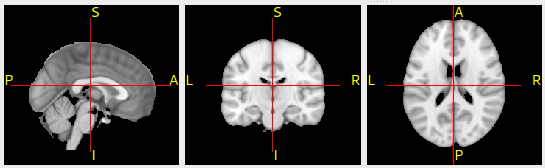
\includegraphics{view_slice2d.png}
\caption{\emph{sagittal plane, coronal plane} and \emph{axial plane} (left to right)}\end{figure}

2D slice view widget sizes can be enlarged by switching the overall layout.
This functionality is implemented in a single button, named \textbf{Switch Layout},
available on the toolbar. By toggling the button, the main view panels switches
between 3D view port and a combination of sliced 2d views.
\begin{figure}[htbp]
\centering

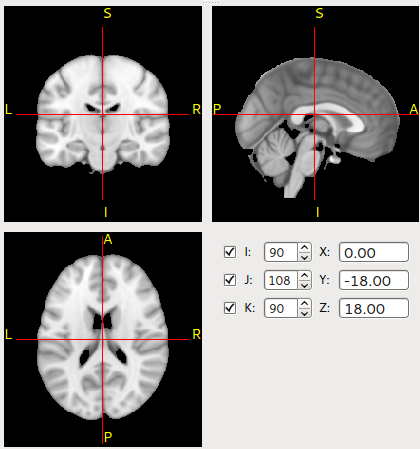
\includegraphics{view_slices.png}
\end{figure}

Image slice index can be changed by clicking on 2d image slice views.
Besides, we perform radiological/neurological (or RAS/LAS) conversion intantly when slice index
values are changed.

For people interested in more details about the radiological/neurological conversion,
please refer to FSL's \href{http://fsl.fmrib.ox.ac.uk/fsl/fslwiki/Orientation\%20Explained}{Orientation Explained} .


\subsubsection{Background Volume Data Layer}
\label{visualization:background-volume-data-layer}
Beginning from this section, several kinds of `layers' are described.
Each `layer' may be contrain one or more data that holds the same property.
By default, the layers manager is located at top-right side of the window.
\begin{figure}[htbp]
\centering
\capstart

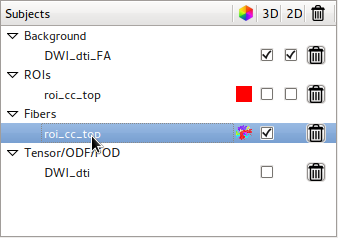
\includegraphics{overlaymgr.png}
\caption{The layers manager}\end{figure}

We refer to \emph{Background} data as plain 3D or 4D volume data that user wants to visualize
its sliced views.
The content should be either a typical 3D image (e.g. T1/T2 image) or a 4D image
such as DWI, DTI, ODF and even fMRI data.

To load a Background Data, click \textbf{Load Background} in the menu or toolbar,
and select a single volume image.
Note that selecting multiple image is not valid here, because the program
doesn't aware which background image is laid that the bottom that might be
overlaid by subsequently loaded images.

Once background image is loaded, several basic data information is shown in the
data property panel.
\begin{figure}[htbp]
\centering
\capstart

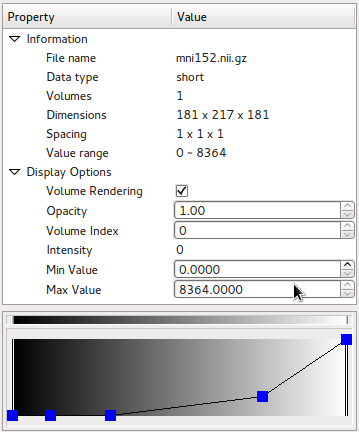
\includegraphics{view_bgprop.png}
\caption{property panel showing mni152 as background image}\end{figure}


\paragraph{Image Contrast Enhancement}
\label{visualization:image-contrast-enhancement}
During loading a Background image, the minimum and maximum intensity values are
calculated and displayed in the data property panel.
By narrow down the range of image intensity values, one can the enhance image contrast.

Note that this functionality is currently applied for 2d sliced views only.


\paragraph{Volume Image Overlay}
\label{visualization:volume-image-overlay}
By loading multiple image throught \textbf{Load Background} menu, one can
This enables the user to make slice to slice comparison to find out image registration errors.

\begin{notice}{note}{Todo}

PUT OVERLAY IMAGE HERE!
\end{notice}


\paragraph{Volume Rendering}
\label{visualization:volume-rendering}
Volume rendering of the background image can be enabled in \emph{Data Property} panel.
Once volume rendering is enabled, a color table is shown to enable users to adjust
color map and opacity values that maps intensity values onto visible planes.
This functionality is particularly useful for visualizing skull-stripped T1 image,
where the folds that increase the surface area of the cortex can be
directly visible without threshold-based surface extraction.
\begin{figure}[htbp]
\centering
\capstart

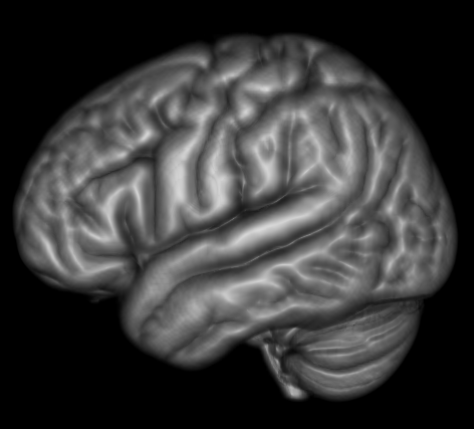
\includegraphics{volrender.png}
\caption{volume rendering of mni152 data}\end{figure}


\subsubsection{Region of Interest (ROI) Layer}
\label{visualization:region-of-interest-roi-layer}
To describe the location of a specific region, we employ the ROI layer.
It outlines surface of the region on 3d view, along with a filled area on 2d slice views.

\begin{notice}{note}{Todo}

compute the voxel-level volume size of a region, as well as its size in millimeters
(by multiplying spacing).
\end{notice}

Once the image data is loaded

Besides, loading multiple ROI data that located within the same directory is allowed.
This saves


\subsubsection{Fiber Layer}
\label{visualization:fiber-layer}

\subsubsection{Tensor/ODF/FOD Layer}
\label{visualization:tensor-odf-fod-layer}

\paragraph{Tensor Data Visualization}
\label{visualization:tensor-data-visualization}

\paragraph{ODF/FOD Visualization}
\label{visualization:odf-fod-visualization}
Due to performance reasons, ODF/FOD is rendered in low resolution by default.
For researchers who need high-resolution images for publication quality results, an option in
the properties panel is provided.


\subsection{Tutorial}
\label{tutorial::doc}\label{tutorial:tutorial}

\subsubsection{Example Data}
\label{exampledata::doc}\label{exampledata:example-data}
We provide a group of test data to test the software, and the data was also used in \footnote{
Xie S., Zuo N., Shang L., Song M., Fan L., Jiang T., 2015. How does B-value affect HARDI reconstruction using clinical diffusion MRI data? PLoS One 10, e0120773.
}.


\paragraph{Basic source for Bash (B-shell) and Python}
\label{exampledata:basic-source-for-bash-b-shell-and-python}
If you want to use script for batch processing, we strongly recommend using Python, since it has nice grammar style and is portable for cross platform.

The Python is easy to learn for basic use as a script language, although its powerful functions largely depend on 3rd party packages. To this end, we have several suggestions to begin with it. First, take a couple of hours to go through the primary Python grammars. There is a large bundle of free but kind tutorials from internet (Google “Python tutorial” or related keywords). You can choose the websites according to your preference. If you are a newbie of Python, don’t think about which version is appropriate for you and just use the latest version (Python\textgreater{}3.0) (In the current stage, you only need to note the difference of “print” function in different versions, which I think is not a smart change from version 3.0); and don’t waste money to buy a book since the materials from the internet are largely beyond your capacity. Several tutorial links are listed here:

For English users
\begin{enumerate}
\item {} 
\href{https://en.wikibooks.org/wiki/A\_Beginner\%27s\_Python\_Tutorial}{https://en.wikibooks.org/wiki/A\_Beginner\%27s\_Python\_Tutorial}, a short tutorial

\item {} 
\href{http://askpython.com/}{http://askpython.com/}, a short tutorial

\item {} 
\href{http://www.learnpython.org/}{http://www.learnpython.org/}, an interactive sandbox

\end{enumerate}

For Chinese users
\begin{enumerate}
\item {} 
\href{http://www.runoob.com/python3/python3-tutorial.html}{http://www.runoob.com/python3/python3-tutorial.html}, a nice tutorial

\item {} 
\href{http://www.cnblogs.com/vamei/archive/2012/09/13/2682778.html}{http://www.cnblogs.com/vamei/archive/2012/09/13/2682778.html}, python and advanced

\item {} 
\href{http://woodpecker.org.cn/abyteofpython\_cn/chinese/}{http://woodpecker.org.cn/abyteofpython\_cn/chinese/}, a complete reference

\end{enumerate}

If you prefer to use shell script, like Bash, you can also find some entrances for tutorials. The shell script itself is easy to follow and it is a powerful tool to concatenate the underlying execution functions. It should be noted that the Bash script is only for * NUX system, so it is not suitable form cross-platforms. Several tutorial links are listed here:

For English users
\begin{enumerate}
\item {} 
\href{http://linuxconfig.org/bash-scripting-tutorial}{http://linuxconfig.org/bash-scripting-tutorial}, a short introduction

\item {} 
\href{http://www.tldp.org/LDP/abs/html/}{http://www.tldp.org/LDP/abs/html/}, a complete tutorial

\item {} 
\href{http://www.learnshell.org/}{http://www.learnshell.org/}, an interactive sandbox

\end{enumerate}

For Chinese users
\begin{enumerate}
\item {} 
\href{http://blog.jobbole.com/85183/}{http://blog.jobbole.com/85183/}, a short tutorial

\item {} 
\href{https://serholiu.com/bash-by-example}{https://serholiu.com/bash-by-example}, several simple examples

\item {} 
\href{http://c.biancheng.net/cpp/view/6998.html}{http://c.biancheng.net/cpp/view/6998.html}, a complete tutorial

\end{enumerate}


\paragraph{How to compute FA/MD/tensor et al for a group subjects?}
\label{exampledata:how-to-compute-fa-md-tensor-et-al-for-a-group-subjects}
Done! Please refer to the diffusionkit/extern/script folder.


\paragraph{How to generate the anatomical connectivity matrix for a given ROI group?}
\label{exampledata:how-to-generate-the-anatomical-connectivity-matrix-for-a-given-roi-group}
Done! Please refer to the diffusionkit/extern/script folder.


\paragraph{Advanced topics: How to generate figures in the paper?}
\label{exampledata:advanced-topics-how-to-generate-figures-in-the-paper}
Done! Please refer to the diffusionkit/extern/script folder \footnotemark[1].

(Xie et al, Journal of Neuroscience Methods, submitted)


\paragraph{Reference}
\label{exampledata:reference}

\subsection{Data Format}
\label{fileformat:data-format}\label{fileformat::doc}\label{fileformat:id1}

\subsubsection{Input}
\label{fileformat:input}
Since we apply the dcm2nii to unify the format of input data,
it can support most types of DICOM files (in folders).
Please refer to the author’s webpage for more information \footnote{
\href{http://www.mccauslandcenter.sc.edu/mricro}{http://www.mccauslandcenter.sc.edu/mricro}
}.
Please also get back to us if you encounter any problems.


\subsubsection{Output}
\label{fileformat:output}
All the intermediate files are in compressed NIFTI format (.nii.gz). The final track file is in .fiber/.fbr or .trk format, where the former is a short version of the later one. The .trk format is from the TrackVis \footnote{
\href{http://trackvis.org}{http://trackvis.org}
}.

The .fiber format is as following

\begin{Verbatim}[commandchars=\\\{\}]
Brainnetome fiber tracking
Version 1
Number\PYGZus{}Fiber 235
Mean\PYGZus{}Length(mm) 150
Volume\PYGZus{}Total(mm\PYGZca{}3)  37020
Mean\PYGZus{}FA  0.6
Mean\PYGZus{}MD  0.07
80 101.378 0.5 0.1
110.758 148.574 124.982 0.166754 0.3
111.253 148.68 123.688 0.198468 0.25
\end{Verbatim}

The first and second line indicates who produces the file and the version of the file format, and line 3 to line 7 characterize several main attributes of this fiber bundle. From line 8, fiber-wise node descriptions are presented; for example, for one fiber on line 8, {[}80 101.378 0.5 0.1{]} corresponds to the total number of nodes, length, mean FA and mean MD of this fiber. Starting from line 9, properties of each node of the fiber are described, e.g., {[}110.758 148.574 124.982 0.166754 0.3{]} denote x-, y- and z-coordinate, FA and MD of this node.


\subsection{Future Improvements}
\label{todo::doc}\label{todo:future-improvements}

\subsubsection{TO-DO list}
\label{todo:to-do-list}\begin{enumerate}
\item {} 
To smooth the ODF/FOD/EAP for a smoother tract;

\item {} 
To add more efficient tracking algorithms;

\item {} 
To optimize the 3D rendering function;

\end{enumerate}


\subsection{Reference}
\label{reference::doc}\label{reference:reference}

\section{Screenshots}
\label{screenshot:screenshots}\label{screenshot::doc}

\subsection{Linux}
\label{screenshot:linux}
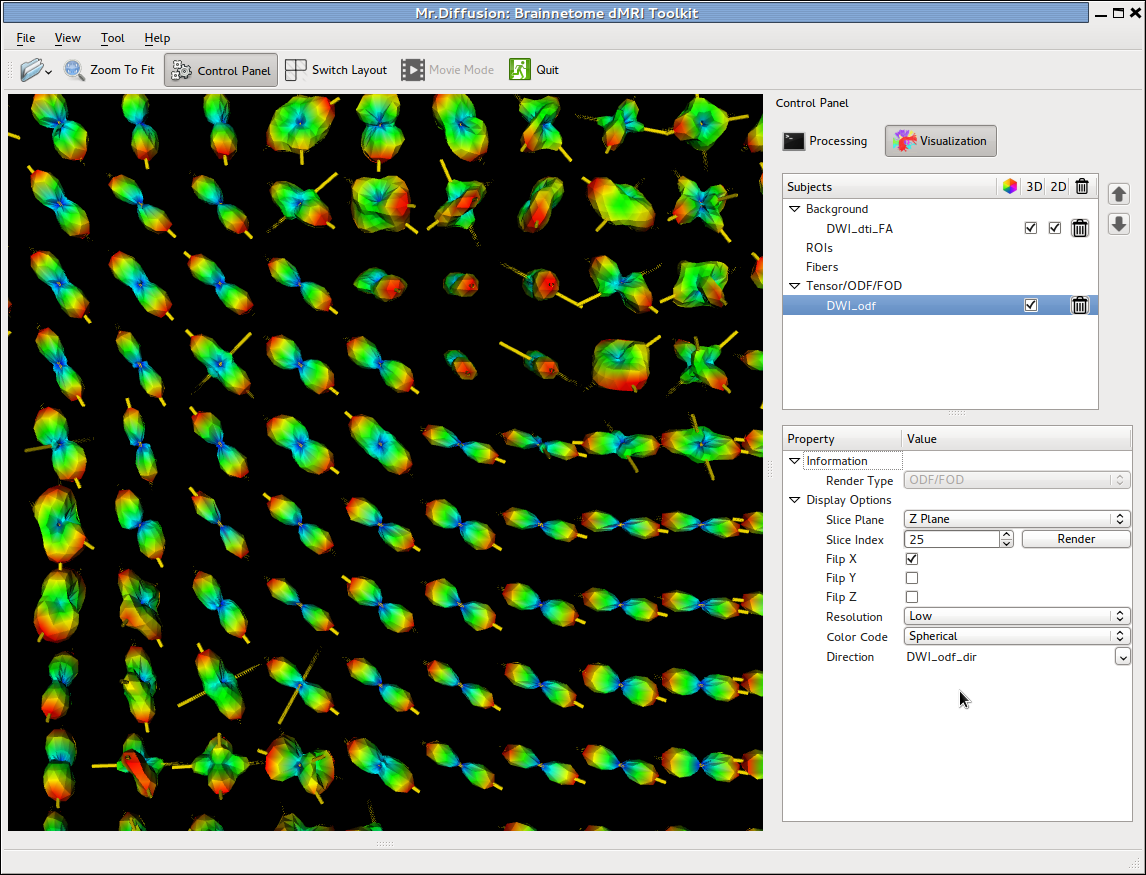
\includegraphics{sticks.png} 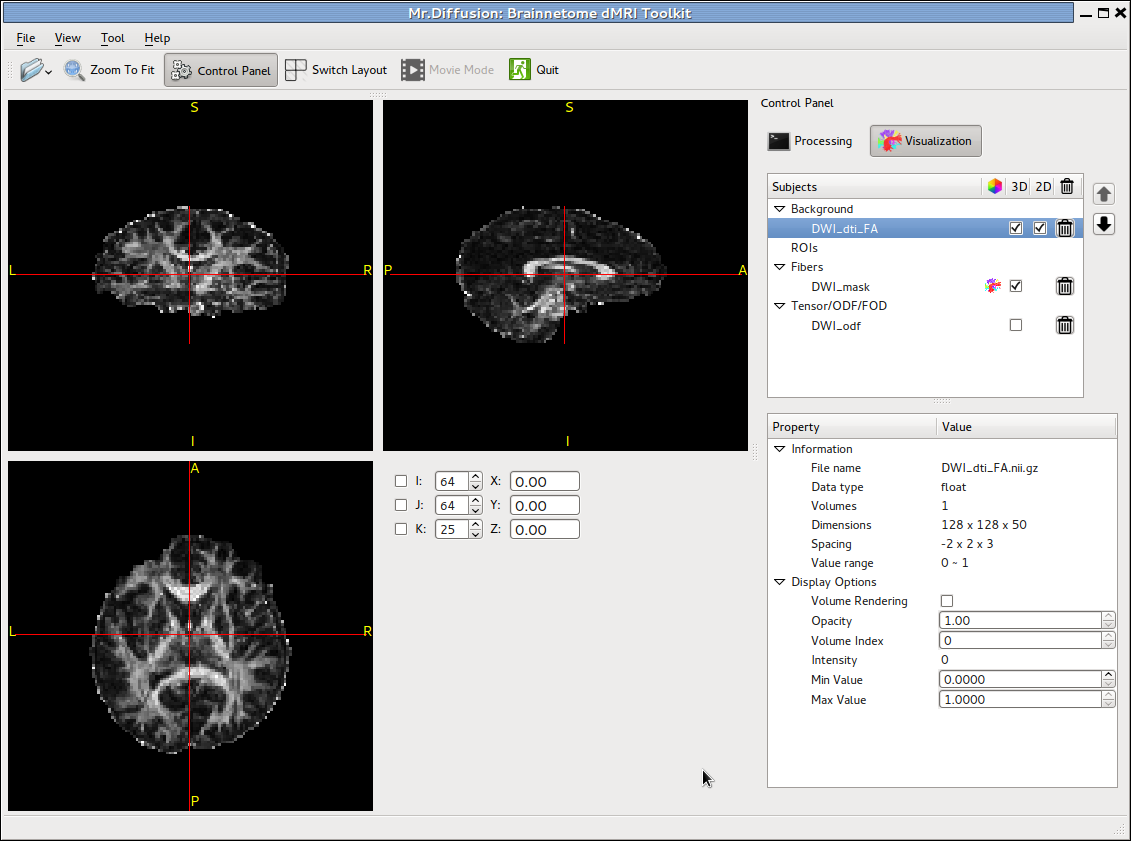
\includegraphics{slices.png}

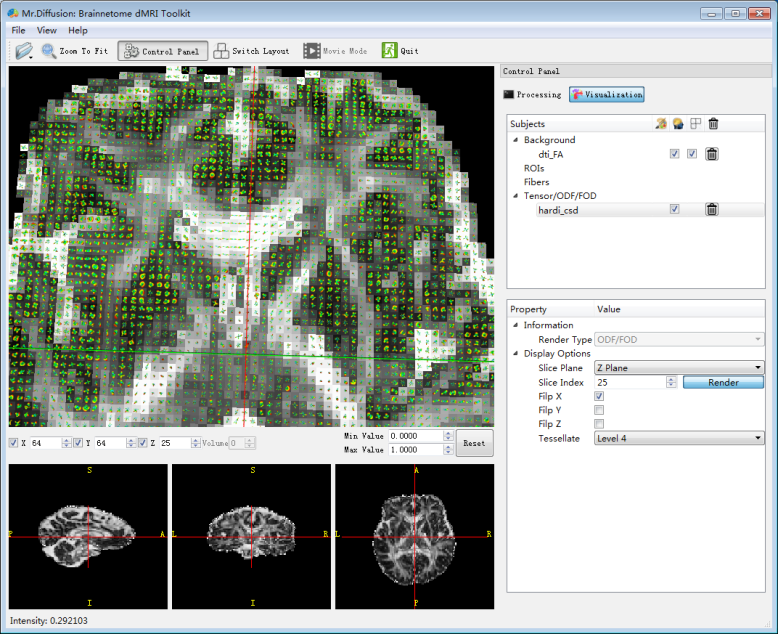
\includegraphics{4A.png} 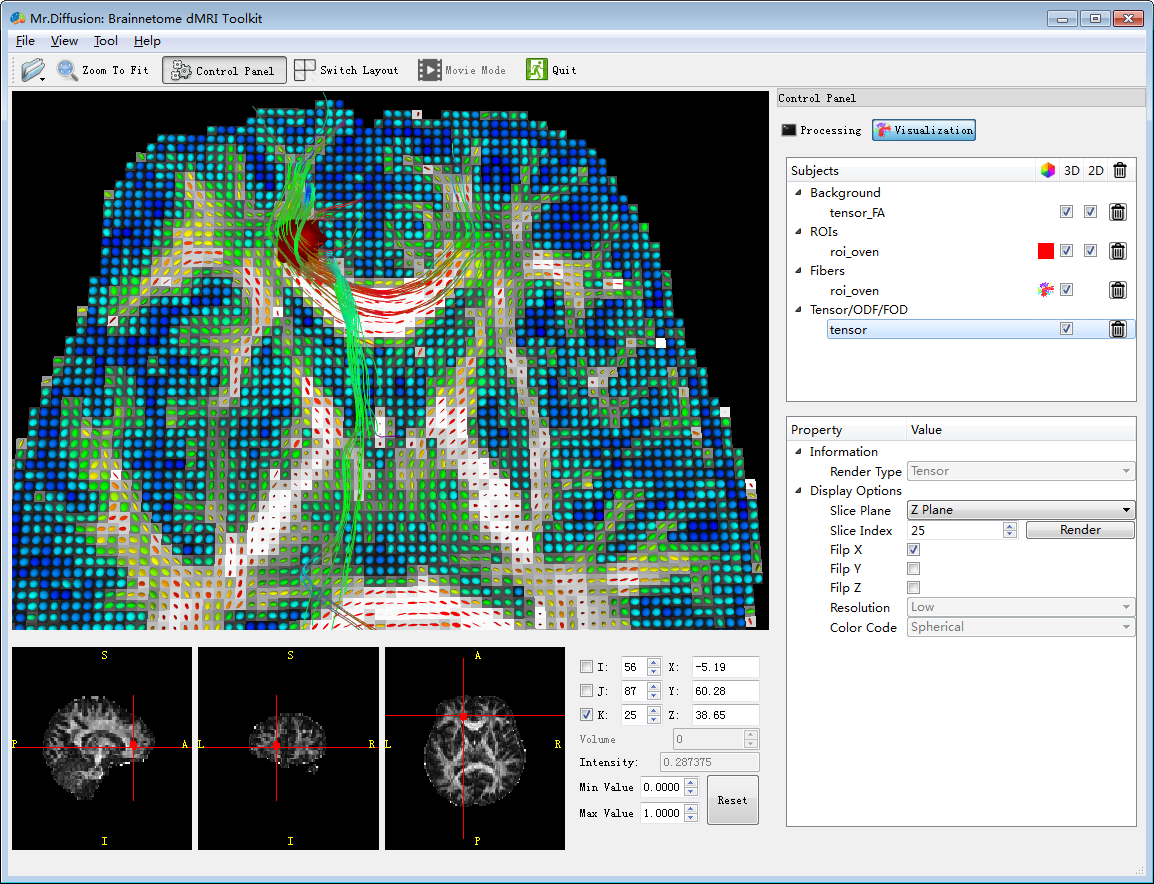
\includegraphics{mainwindow.png}

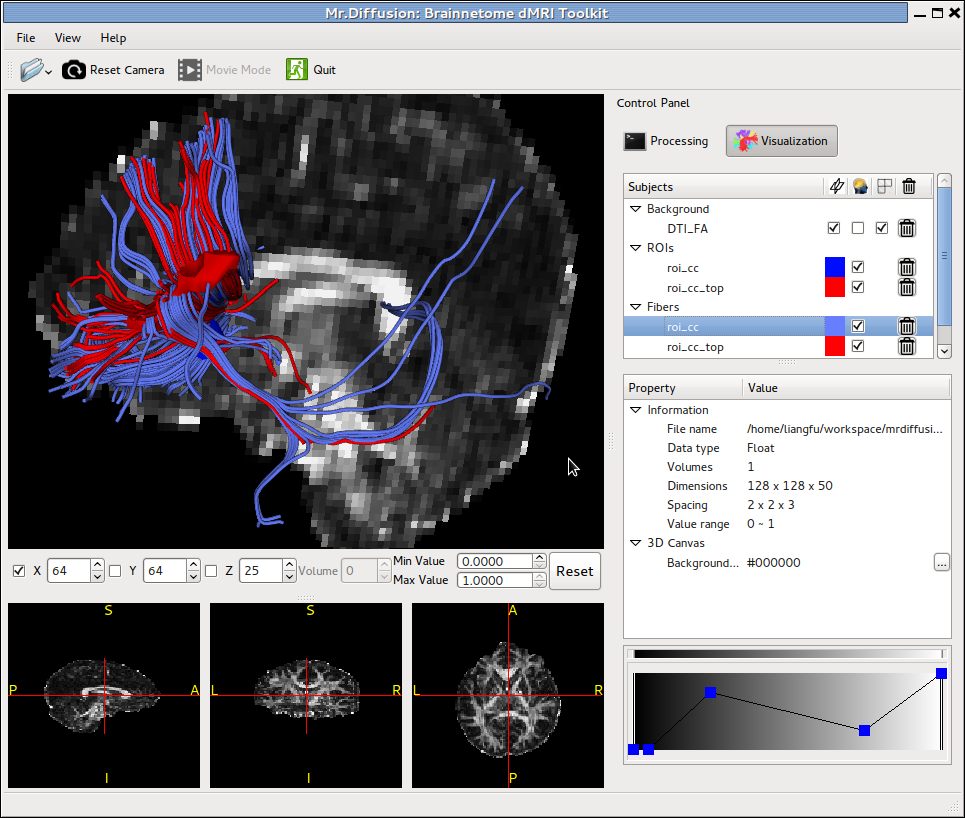
\includegraphics{fibers.png} 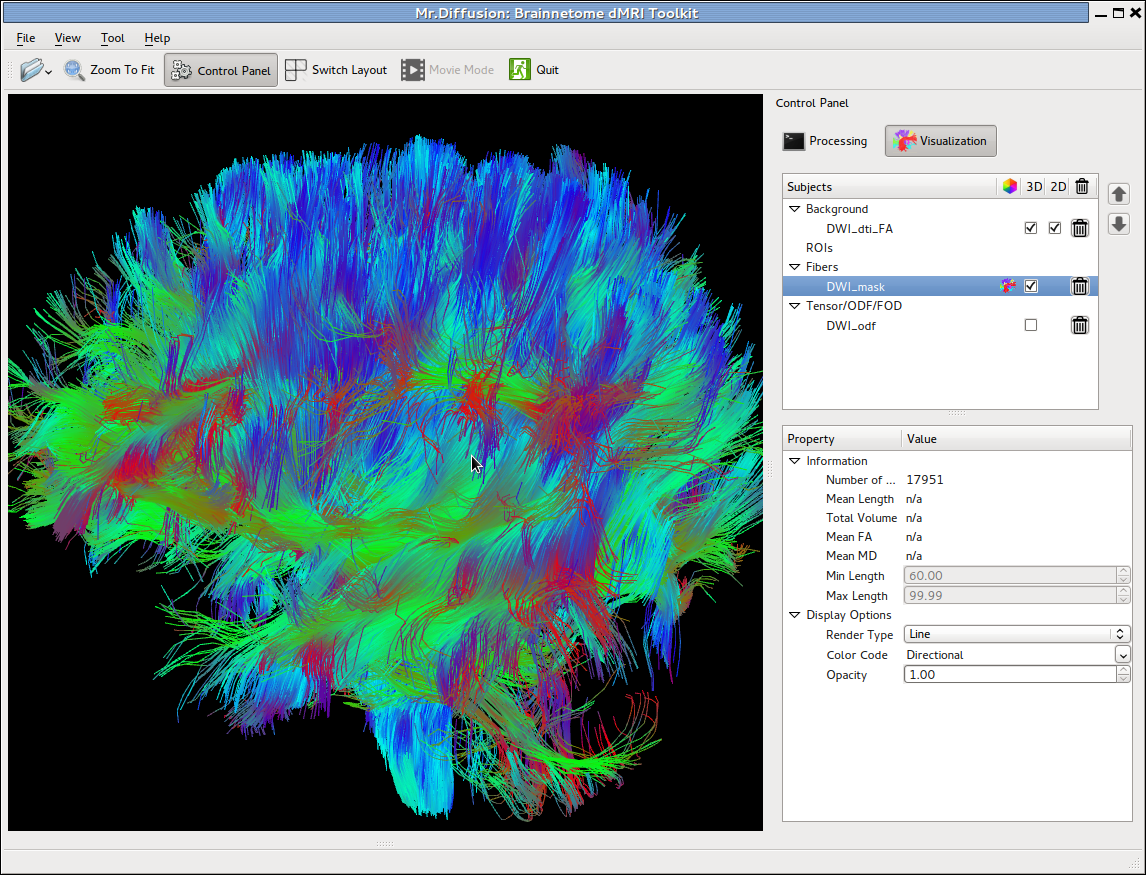
\includegraphics{fibers2.png}


\subsection{Windows}
\label{screenshot:windows}

\section{Download}
\label{download:download}\label{download::doc}

\subsection{Download Links}
\label{download:download-links}

\includegraphics{winlogo.jpg} \href{https://github.com/liangfu/diffusionkit/releases/download/v1.1/DiffusionKitSetup-WIN64-v1.1.exe}{Windows Installer (x86-64)}


\includegraphics{winlogo.jpg} \href{https://github.com/liangfu/diffusionkit/releases/download/v1.1/DiffusionKitSetup-WIN32-v1.1.exe}{Windows Installer (x86)}


\includegraphics{rellogo.jpg} \href{https://github.com/liangfu/diffusionkit/releases/download/v1.1/DiffusionKitSetup-x86\_64-v1.1.tar.gz}{Linux Binary Package (x86-64)}


\subsection{System requirement}
\label{download:system-requirement}
Basically this software can run in any system, including 32/64-bit MS Windows/Linux OS,
although currently we only tested and released the binary packages for Windows/Linux OS.
The software is developed based on C/C++, and some platform independent packages,
including ITK, VTK, and OpenCV, etc.
However, for high-performance data processing and visualization,
we recommend using 64-bit OS with multi-core CPU and standalone video card.


\subsection{Install/Uninstall}
\label{download:install-uninstall}
Please download the package from \href{http://diffusion.brainnetome.org}{http://diffusion.brainnetome.org} ,
according to your own OS. Unpack the files to where you want and you can enjoy the software.
The 64-bit OS is recommended for high-performance data processing.
Each installation package is completely standalone so you DO NOT need to
install ANY other dependency to run the software.
If you encounter any dependency problem please DO \href{mailto:diffusion.kit@nlpr.ia.ac.cn}{contact us}.


\subsubsection{For MS Windows OS}
\label{download:for-ms-windows-os}
Double click the \code{DiffusionKitSetup-v1.1.exe} file and then choose the destination path
according to the wizard. You may need to provide administrator permission
if you want to put the files into the system path.
Similarly, to uninstall you only need to hit the menu of “uninstall” in the MS Windows start menu.


\subsubsection{For Linux OS}
\label{download:for-linux-os}
\code{Glibc\textgreater{}=2.2} is required. Download the \code{DiffusionKitSetup-v1.1.tar.gz}, and then

\begin{Verbatim}[commandchars=\\\{\}]
tar zxvf DiffusionKitSetup\PYGZhy{}v1.1.tar.gz
\PYG{n+nb}{cd }diffusionkit/bin
./bnviewer \PYG{c}{\PYGZsh{} (you can run the command in this way)}
\end{Verbatim}

If you do not want to type the full path every time, you could add the path to the \$PATH. Edit the \textasciitilde{}/.bashrc file, then add the following line,

\begin{Verbatim}[commandchars=\\\{\}]
\PYG{n+nb}{export} \PYG{n+nv}{\PYGZdl{}PATH}\PYG{o}{=}\PYG{n+nv}{\PYGZdl{}PATH}:/your/path/to/diffusionkit
\end{Verbatim}

To uninstall the software, just manually remove the entire folder where you untar-ed the .tar.gz file.

That’s it! Enjoy the software now!


\section{License}
\label{license::doc}\label{license:license}
Copyright ©  2013-2015 \href{http://www.brainnetome.org/}{Brainnetome Center}, CASIA

This software is provided `as-is', without any express or implied warranty.
In no event will the authors be held liable for any damages arising from the use of this software.

Permission is granted to use this software for any purpose,
including research purpose and commercial applications, subject to the following restrictions:
\begin{enumerate}
\item {} 
The origin of this software must not be misrepresented; If you use this software in your work, an acknowledgment is required. A written permission is also required for commercial use.

\item {} 
Altered versions must be plainly marked as such, and must not be misrepresented as being the original software.

\item {} 
This notice may not be removed or altered from any distribution.

\end{enumerate}


\section{Support}
\label{feedback:support}\label{feedback::doc}

\subsection{Feedback}
\label{feedback:feedback}
If you encounter any problems or have any suggestions,
please feel free to get back to us, \href{mailto:diffusion.kit@nlpr.ia.ac.cn}{diffusion.kit@nlpr.ia.ac.cn} .

\begin{notice}{note}{Note:}
Document last updated on November 24, 2015.
\end{notice}


\section{Reference}
\label{index:reference}


\renewcommand{\indexname}{Index}
\printindex
\end{document}
